\chapter{Introduction}\label{ch:intro}

\section{Shaping the Universe with Massive Stars} % (fold)
\label{sec:massive_stars}
Understanding how stars form and evolve is fundamentally important to understanding the physical processes which govern the Universe.
As congregations of stars are built up they form heavily structured galaxies where the complex internal interactions between stars and gas, as well as the underlying stellar population, are vitally important to the chemical and dynamical evolution of the galaxy~\citep[e.g.][]{2014ARA&A..52..291C}.
Stars die to produce black holes where massive stars are good candidates for producing the recently observed gravitational wave signature~\citep{2016PhRvL.116f1102A,2016arXiv160204735L,2016arXiv160300511W} and fundamentally, stars are at the heart of almost every area of study in astrophysics: from active galactic nuclei to exoplanets, solar system bodies to high-redshift galaxies; an understanding of stars and stellar evolution is vital in understanding these different phenomena.

Stars form with various masses ranging from the hydrogen fusion limit of $\sim$0.08\,M$_{\odot}$~\citep{1997ApJ...491..856B,2000ARA&A..38..337C} to an uncertain upper mass limit in excess of $\sim$100\,M$_{\odot}$~\citep[e.g.][]{2005Natur.434..192F,2012MNRAS.422..794E,2014A&A...568L..13W} and up to $\sim$300\,M$_{\odot}$ in extreme cases~\citep{2010MNRAS.408..731C}.
Massive stars~\citep[defined here as stars with initial masses $>$8\,M$_{\odot}$ e.g.][and expanded upon in Section~\ref{sec:lives}]{2014ARA&A..52..487S} are probably the most important type of star with respect to how they shape their surrounding environments throughout their lives and distribute chemical elements in their deaths.
Massive stars drive the ionisation of their surrounding birth cloud and are good candidates for the reionisation of the Universe~\citep[e.g.][]{1997ApJ...483...21H,2005SSRv..116..625C,2006ARA&A..44..415F}.
During the short lifetime of a massive star (detailed in Section~\ref{sec:lives}) massive stars expel material from their outer layers in strong winds at various evolutionary stages throughout their lives.
These winds help to distribute nuclear processed material throughout their parent galaxies and pollute the interstellar medium (ISM) with heavy elements.

In any given star-forming galaxy, the massive-star population dominates the light output across the full spectrum of light.
Ultraviolet and optical light is dominated by hot massive stars~\citep{1998ARA&A..36..189K,2012ARA&A..50..531K} with temperatures of up to 50\,000\,K~\citep[e.g.][]{2011A&A...530L..14B}.
Whereas infrared light is dominated by the cool (4000\,K) evolutionary products of these hot massive stars, i.e. red supergiant stars (RSGs), which can be as luminous as entire galaxies in the near infrared (near-IR).

Given that massive stars are extremely luminous, they can be identified in extra-galactic systems at large distances.
Indirectly, by ionising their surrounding birth cloud, massive stars are used to study galaxy populations at early epochs of the Universe~\citep{2004MNRAS.348L..59P}.
In the more local Universe, massive stars can be used to probe the structure and chemical evolution of galaxies in great detail~\citep{2007ApJ...659.1198E,2008ApJ...681..269K,2008MNRAS.386..826E,2010AN....331..459K,2011A&A...530A.108E,2012A&A...542A..79C}.

In this thesis I expand and develop the methods by which we can study massive stars (in particular RSGs) in extragalactic environments.
The study of RSGs in external galaxies spans two key astrophysical topics: stellar evolution and galaxy evolution.
By using RSGs as abundance probes I have been able to map the spatial distribution of metals in external galaxies as well as gain insight into the underlying physics which is used within evolutionary and atmospheric models.

In the coming years, RSGs will play a more central role in the study of extragalactic systems owing to their extreme brightness coupled with the fact that their peak luminosity is in the near-IR. Given the intrinsic advantages with dust extinction in the near-IR, this is particularly poignant when considering that the next generation of ground- and space-based telescopes will be optimised for study in this wavelength regime.

% subsection massive_stars (end)

\section{The Lives of Massive Stars} % (fold)
\label{sec:lives}

Stellar evolution is critically dependent upon the initial mass of the star.
A 10\,M$_{\odot}$ star has a very different evolutionary path to that of a solar mass star.
Their formation, subsequent evolution and eventual fate all depend upon how much mass the star is able to accumulate during its formation.
Therefore, an understanding of how massive stars are able to gather their mass is crucial to the understanding of how these objects evolve and end their lives.
To this end, I provide an outline of the main process by which star formation occurs (focussing on massive stars) in Section~\ref{sub:birth}. Section~\ref{sub:life_cycle} describes the evolution of a massive star after the onset of hydrogen-burning in the core up until the final stage of evolution before the star ends its life.
This leads onto Section~\ref{sub:death} which reviews the eventual fate of massive stars.

\subsection{Birth} % (fold)
\label{sub:birth}

Massive stars, as with lower mass stars, begin their lives within giant molecular clouds (GMCs), which are regions consisting of large clumps of interstellar material which have become over-dense with respect to the surrounding interstellar medium.
These clouds are typically 10$^{4}$--10$^{7}$\,M$_{\odot}$, extend over 50--100\,pc and represent the densest parts of the interstellar medium~\citep{Fukui10}.
In a high-mass molecular cloud, high- and low-mass star formation takes place.
Studies suggest that as the mass of the cloud decreases, so does the mass of the largest stars~\citep{Fukui10,Weidner10}; however, some studies suggest that this may not be a universal property~\citep[e.g.][]{Bressert12}.

Within GMCs, over-dense regions continue to grow and eventually fragment into smaller cores.
If these dense cores consist of a region where the local mass is greater than the associated Jeans mass for the region, the region is unstable to gravitational collapse.
As the region collapses into a protostellar core, the optical depth increases, which gives rise to a large increase in temperature~\citep{Zinnecker07}.
The collapse proceeds until the radiation pressure exerted by the core is able to resist the gravitational collapse.
The system is now in hydrostatic equilibrium and evolution proceeds though accretion.
The collapsed core accretes matter from a surrounding disk which has condensed around the protostar.
Meanwhile, the core of the protostar contracts and increases the temperature of the core towards hydrogen-burning temperatures.
A larger protostar can accrete a larger amount of additional material from its surroundings and in turn grows to become a more massive star.
In lower mass stars, accretion ceases before the star reaches the main sequence; however, a more massive star can perturb a larger amount of material and hence continues to accrete matter even after the hydrogen-burning phase has begun in its core.
The ignition of hydrogen ends the period of formation, as the star now has a central energy source which governs the evolution for the remainder of time spent on the main sequence.
However, massive stars have one more crucial role to play in the process of star formation.
Massive stars end their lives as supernovae, ejecting fusion products back into the environment from which they were born.
The surrounding gas is shocked and compressed by this mass ejection event which can be the catalyst needed to produce more star formation in these environments (triggered star formation).
% Jeans Mass is the maximum mass a cloud of gas can have before it becomes unstable to gravitational collapse
% Optical depth is a measure of how much light is not dispersed in the line of sight I=I_{0}e^{-\tau}

This is a very simplistic, qualitative overview of the formation of massive stars.
In reality the exact processes governing these main stages of formation are complicated by various factors, for example, the effect of turbulence has been completely neglected in this discussion but has a vital role in many phases of star formation~\citep{McKee07}.
The relative importance of each of the processes involved is not well understood.
As of yet, there is no universal theory of how star formation proceeds in massive stars.

There are several crucial differences between low- and high-mass star formation.\footnotemark~
\footnotetext{The opinion in the literature seems to suggest that low-mass star formation continues as normal up until around $\sim$20\,M$_{\odot}$~\citep{Zinnecker07, Crowther12}, above this, star formation must take into account various complicating factors (see text).}
Massive stars have larger temperatures and hence produce a large amount of ionising photons.
This means that the accretion disk and outer envelope surrounding the massive star is photoevaporated and dissociated through interactions with these high energy photons.
As alluded to previously, massive stars continue to accrete matter while on the hydrogen-burning main sequence~\citep{Zinnecker07}
whereas lower mass stars ($<$0.2\,M$_{\odot}$) spend at least 10\,Myr evolving towards hydrogen fusion~\citep{Luhman12}.
A key difference in the star formation across a large mass range is the role of accretion.
In lower mass star formation, accretion does not form significant amounts of the final mass of the star~\citep{Bonnell08}, whereas in higher mass star formation, accretion is generally accepted as a key role in accumulating the mass of the star~\citep{Kraus10}.


Exactly how accretion acts is subject to much debate.
Accretion is likely to proceed via competitive accretion~\citep{Bonnell01}.
This is where a large fraction of the star is accreted from its surrounding material.
In this scenario, the amount of material available for accretion is limited only by the surrounding environment.
A star at the centre of the potential well of the surrounding gas cloud will be able to accrete more material than a star on the outskirts and hence will grow larger.
As the star grows larger, it is able to accrete more and more matter.
Eventually, neighbouring stars will be forced to compete for the surrounding gas, and in this scenario, the largest star (i.e. the star at the centre of the potential well) will be able to accrete a larger amount of material~\citep[for a useful economical analogy -- the rich get richer --, see Section 4.2 of][]{Zinnecker07}.
In competitive accretion theory, the mass of the star is determined entirely by the environment in which it resides in and not by the initial conditions of the collapse.

Other theories of massive star formation in this context are those presented by~\cite{Yorke02}, where accretion occurs onto the protostar via a disk which is produced as a result of the monolithic collapse of the gas cloud (into the protostar).
In this scenario, the mass of the star is limited to the combined total of the protostar and the accretion disk~\citep{Zinnecker07}.
However, this theory has difficulty explaining the observed multiplicity and clustering of massive O stars~\citep{Zinnecker07, Sana12, 2012ARA&A..50..531K}.

An alternative path (which explains the formation of the most massive stars) is through stellar collisions.
During the merging of star clusters, where stellar densities are highest, massive star formation can proceed through stellar collisions, resulting in very massive stars concentrated at the centre of clusters~\citep{Fujii13}.


%% Runnaway OB stars make up around 10-25% of the population of OB stars, however these stars are thought to have formed within a cluster~\citep{Zinnecker07}

% subsection birth (end)
\subsection{The Circle of Life} % (fold)
\label{sub:life_cycle}

All stars spend a majority of their active life fusing hydrogen to helium in their cores on the hydrogen-burning main sequence (MS).
On the MS, all stars remain in a stable state of hydrostatic equilibrium and hence their evolution in terms of luminosity and temperature is small~\citep{2012sse..book.....K}.
Once massive stars exhaust their core hydrogen fuel, various stages of nuclear burning succeed, including core helium- and carbon-burning.
During this evolution, the surface temperature decreases and stars appear increasingly redder at later stages of their evolution.
This evolution is typically characterised on a Hertzsprung-Russell (H--R) diagram which is a diagram relating the surface temperature against the luminosity of a star and can be used to illustrate how the appearance of stars change throughout their lives.
Figure~\ref{fig:HRD} displays a H--R diagram which shows stellar evolutionary models of stars of various masses, in black lines.
Initial masses (in Solar units) of some of the important distinctions in stellar evolution are labelled at the start of their respective models.
The 7\,M$_{\odot}$ evolutionary model is labelled with five red points indicating important transitions in its evolution.
Each model begins at the onset of hydrogen fusion (point 1) within the core of the star and when viewed in comparison with other models at different initial masses forms the MS of stellar evolution.
Once stars exhaust their fuel in the core they cool and evolve off the MS (towards the right in Figure~\ref{fig:HRD}) and depending upon their masses, go on to fuse heavier elements in their cores.
The models shown in Figure~\ref{fig:HRD} end at the exhaustion of carbon burning in the core (if applicable; point 5).


\begin{figure}
 \centering
 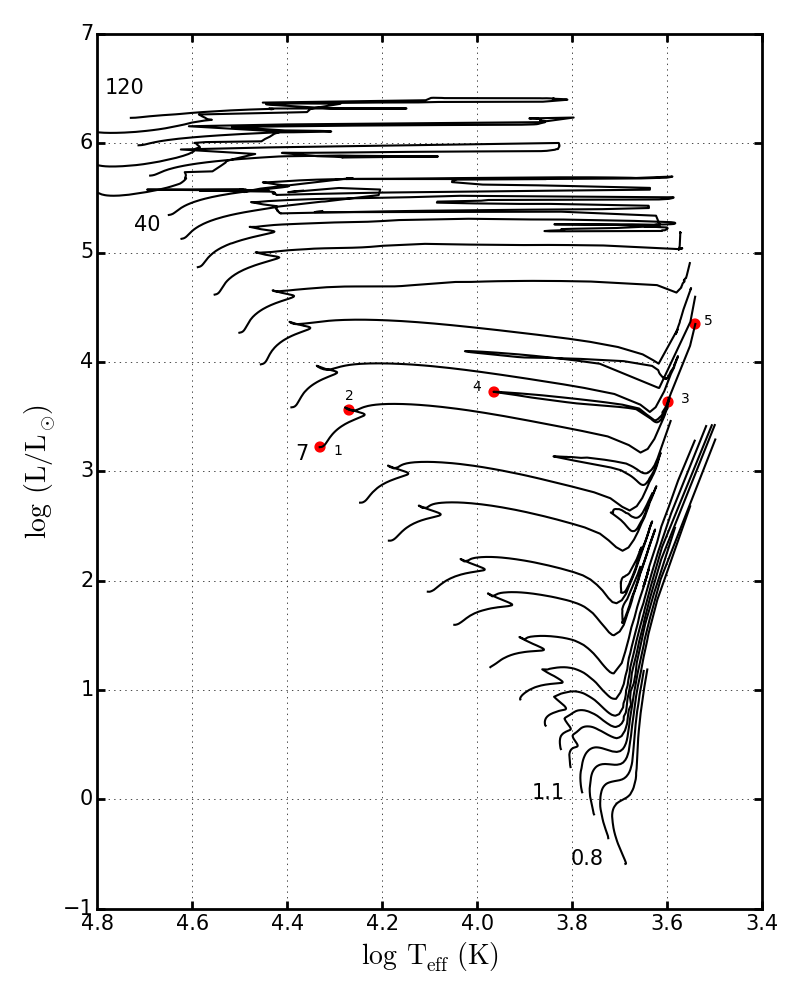
\includegraphics[width=0.75\textwidth]{intro/HRD-geneva}
 \caption[Hertzsprung-Russell (H--R) diagram of stars]{
Hertzsprung-Russell (H--R) diagram displaying the surface temperature (increasing to the left) against luminosity of stellar evolutionary models in the mass range
0.8~$<$~M/M$_{\odot}<$~120 using evolutionary models from
\protect\citet{2012A&A...537A.146E}.
Each line represents a model, at Solar-like metallicity computed without stellar rotation.
Initial masses of some important transition regions are given to the left (i.e. the start) of the models.
Red points on the 7\,M$_{\odot}$ track mark important changes within a stars lifetime:
1. Onset of hydrogen fusion (start of models),
2. Exhaustion of fuel in the core,
3. Onset of helium core fusion,
4. Blue loop,
5. End of core carbon fusion (end of model).
Stars spend most of the lives on the left hand side of this diagram on what is commonly known as the main sequence (MS) of stellar evolution.
After exhausting the hydrogen fuel in the core, the star becomes more extended and hence cools and is said to appear ``redder'' (toward the right of the diagram).
See text for more details on these phase of evolution.
 \label{fig:HRD}}
\end{figure}


During core hydrogen-burning, stars more massive than 1.1\,M$_{\odot}$ fuse hydrogen to helium through the carbon-nitrogen-oxygen (CNO) cycle.
In this case, convection is induced in the core owing to the large temperature gradient established as a result of the high temperature dependence of the rate of the CNO cycle (T$^{14}$).
As a result of convective mixing, the core can be described as homogeneous during the hydrogen-burning phase~\citep{2012sse..book.....K}.
Convection is an important feature of this stage of evolution as it increases the MS lifetime by increasing the amount of material available for fusion.

Some of the main issues with the current theory of convection are characterising the size of the convective overshoot region and the effects of semi-convection on stellar evolution.
Convective overshooting acts to increase the mixing of material beyond the convective boundary, within a stable region.
As a convective cell is accelerated towards the boundary of the convective layer, its momentum carries the cell beyond this region into a region of convective stability.
This has several consequences for the evolution of the hydrogen-burning phase, which are direct results of convective overshooting increasing the amount of fuel available for consumption within the convective core.
How large an evolutionary effect convective overshooting produces is not well constrained.

Convective overshooting is characterised by the parameter $\alpha$ in units of the local pressure scale height ($H_{P}$)~\citep{2012sse..book.....K}.
% What is the local pressure scale height?
Various authors have placed constraints upon $\alpha$ by using observational techniques including, for example, measuring the width of the main sequence~\citep{Schroder97,Brott11}.
These studies find values of $\alpha$~=~0.1--0.6~\citep[e.e.][who found $\alpha = 0.335$]{Brott11}.

In addition to the uncertainties surrounding the convective overshooting problem, as the opacity in massive stars in dominated by electron scattering~\citep{b:Bohm-vitense92.v3}, outside a fully convective core, semi-convection occurs.
Semi-convection is a discrepancy between two the criteria for convection outside a fully convective zone where a chemical gradient ($\nabla _{\mu}$) is established.
Semi-convection acts to smooth out the chemical gradient outside the fully convective regions and can determine how the star evolves and ends its life after this phase~\citep[e.g.][]{1989A&A...224L..17L}.

As the star evolves and more hydrogen is consumed, the mass of the convective core decreases~\citep{2012sse..book.....K}.
Eventually, the star consists of a pure helium core surrounded by a hydrogen-burning shell.
The maximum mass of the helium core, with respect to the total stellar mass is determined by the Sch\"onberg-Chandrasekhar limit
(q$_{SC}\geq\frac{M_{c}}{M_{tot}}$; usually derived as q$_{SC}\sim$~0.1), above which an inert helium core is unstable to gravitational collapse.
In stars in the mass range 3~$<$~M/M$_{\odot}<$~12, the Sch\"onberg-Chandrasekhar limit is usually reached at the end of the hydrogen-burning phase~\citep{b:SalarisCassisi05}.
At this point, the helium core collapses, increasing the core temperature and density sufficiently that core helium-burning can occur, halting the collapse in the process.
In more massive stars ($>$12\,$M_{\odot}$), core helium-burning can smoothly proceed without the need for core collapse, as the central temperature in these stars is sufficiently high (10$^{8}$\,K).

During this phase of evolution hydrogen-burning proceeds within a shell outside the core.
For stars which exceed the Sch\"onberg-Chandrasekhar limit, during core contraction the outer hydrogen envelope will expand owing to the ``mirror principle'' of shell fusion~\citep[e.g.][]{2012MNRAS.421.2713B}.\footnotemark
As the outer envelope expands, the effective temperature decreases.
In Figure~\ref{fig:HRD}, the star moves to the right (towards redder colours) where massive stars evolve into the RSG phase and lower mass stars become red giant branch stars.
This phase of evolution proceeds on a Kelvin-Helmholtz timescale, which for a 7\,M$_{\odot}$ star is around 5~$\times$~10$^{5}$\,yr~\citep{2012sse..book.....K}, i.e. incredibly short on an evolutionary timescale.
% The short timescale on which this evolutionary phase proceeds accounts for the observed Hertzsprung gap.
The evolution towards the red is halted as core helium-burning switches on.
\footnotetext{This principle is not well understood, but its effects appear to be a universal feature of shell fusion~\citep{2000ApJ...538..837S,2009PASA...26..203S,2012MNRAS.421.2713B}.}


In massive stars above 12\,M$_{\odot}$, core helium-burning is thought to ignite when the star appears as a blue supergiant (BSG)~\citep{Meynet11,2012A&A...537A.146E,Langer12,Saio13}.
The redward migration of BSG stars is dictated by an intermediate convective zone~\citep{Meynet11} present in the atmosphere of the star, and is more gradual than the redward evolution of less massive stars.
Stars more massive than around 40\,$M_{\odot}$ never become RSGs~\citep{Massey03,Meynet11,2012A&A...537A.146E} and hence, there is a peak luminosity of RSGs in any given population~\citep{1979ApJ...232..409H}.
As these massive stars evolve towards the red edge of the H--R diagram, their luminosities approach that of their Eddington luminosities; this induces large mass loss episodes.
As a result, these stars halt their evolution towards the RSG phase and evolve towards the blue and consequently into Wolf-Rayet (WR) stars
\citep{2007ARA&A..45..177C, Vink09}, see 60\,M$_{\odot}$ track and above in Figure~\ref{fig:HRD}.

% For a 10M$_{\odot}$ star, core helium-burning proceeds for around 4Myrs~\citep{b:SalarisCassisi05}.
As suggested above, in specific cases, not all of the helium-burning phase is spent as a RSG.
The length of time spent during the RSG phase depends upon how core helium-burning ignites.
If a star begins its helium-burning lifetime as a BSG and subsequently evolves into the RSG phase, naturally, the length of time spent as a RSG will be shorter.
In addition to this, stars with masses in the range of 25~$<$~M/M$_{\odot}<$~40 are thought to evolve back from the RSG phase to the BSG phase while still burning helium in their cores~\citep{2012A&A...537A.146E}.

This evolution of massive stars between the BSG and RSG phase seeds the idea that stars in these stages of evolution will fall into two categories:

\begin{enumerate}
    \item stars which begin helium-burning in the RSG or BSG phase, or,
    \item stars which begin helium-burning in a different evolutionary state and have since evolved into either the RSG or BSG regime.
\end{enumerate}

Distinguishing these objects observationally is challenging.
\cite{Saio13} used radial pulsations to distinguish between models of BSGs, which \textquoteleft roughly agree\textquoteright ~with observations of NGC 300 and in the Galaxy.
However, an analogue to this has not been identified in RSGs.
\cite{2012A&A...542A..79C} argued based on the nitrogen enrichment of their population of observed BSGs that these stars are in the process of evolving toward a RSGs phase.
The ratio of BSG/RSG is used as a test of stellar evolutionary model which has been an issue for some time~\citep{1995A&A...295..685L} and is known to be affected by rotation~\citep{2001A&A...373..555M,2012A&A...537A.146E} and binarity~\citep{2008MNRAS.384.1109E}.


Regardless of how extended the external envelopes in these stars are, core helium-burning proceeds through the triple alpha process, via the reaction, 3$\alpha$~$\rightarrow$~$^{12}$C~+~$\gamma$.
However, as the number density of $^{12}C$ increases, the reaction $^{12}$C($\alpha+\gamma$)$^{16}O$ is of increasing importance, although the exact rates at which these reactions proceed is not well constrained.
This process of nuclear burning is highly temperature sensitive (even more so than the CNO cycle); therefore convection within the core is once again established.
In addition to this, massive red helium-burning stars also have large outer convective envelopes~\citep{2012sse..book.....K} and as a result of this the star appears near the Hayashi limit for a fully convective star in the H--R diagram.
The Hayashi limit is a limit on the coolest surface temperature a star can have as beyond this, the star is no longer in hydrostatic equilibrium~\citep{1961PASJ...13..442H}.
The convective envelope dominates the evolution of all but the most massive RSGs (30~$<$~M/M$_{\odot}<$~40) which do not not appear as close to the Hayashi limit as their lower mass counterparts~\citep[see Figure 1 in][]{Saio13}.

At the end of the core helium-burning phase, a massive star contains a carbon/oxygen core surrounded by a helium-burning shell, which is in turn surrounded by a hydrogen-burning shell.
At this point, the situation in the core now resembles that of the stage before core helium-burning.
An inert carbon/oxygen core contracts and heats up which ignites the core fuel.
Stars with initial masses greater than around 8\,M$_{\odot}$ are able to fuse carbon in their cores in a stable fashion.
In order for lower mass stars to do so, a degenerate carbon core is required.
Whether or not stars are able to begin core carbon-burning in a stable manner is usually the physical basis for distinguishing between ``intermediate'' and ``high'' mass stars.
During this process, carbon fuses to form an unstable form of $^{24}$Mg which then decays through three channels:

\begin{enumerate}
    \item $^{24}$Mg$^{*}\rightarrow ^{23}$Mg$+n+\gamma$,
    \item $^{24}$Mg$^{*}\rightarrow ^{20}$Ne~+~$\alpha+\gamma$,
    \item $^{24}$Mg$^{*}\rightarrow ^{23}$Na~+~$p+\gamma$.
\end{enumerate}

Oxygen does not fuse at this stage of the evolution of the star and therefore the length of time a star spends fusing carbon depends strongly on the amount of carbon processing present in the helium-burning phase and hence, the reaction $^{12}$C($\alpha+\gamma$)$^{16}O$.

Once the carbon fuel has been exhausted in the core, shell carbon-burning proceeds.
The cycle of core contraction with new core reactants begins and subsequent neon-, oxygen- and silicon-burning in the core follow~\citep{Woosley02}.
As each new fuel in the core is exhausted, shell burning follows.
Fusion reactions cease with $^{56}$Fe as fusion reactions beyond this point are no longer energetically favourable.

Eventually, this leads to an \textquoteleft onion structure\textquoteright
~star, with an inert iron core surrounded by layers of lighter elements fusing in shells.
These fusion reactions proceed on such a short timescale that the outer envelope does not have the time to react to the changing conditions in the core.
This effectively \textquoteleft freezes out\textquoteright ~the outer envelope and the spectral type of the star does not change significantly during this period~\citep{Meynet11}.

% subsection life_cycle (end)

\subsection{Death} % (fold)
\label{sub:death}

Massive stars ($>$8\,M$_{\odot}$) end their lives as core-collapse supernovae (CCSN).
These violent explosions distribute elements synthesised within massive stars during their nuclear-burning lifetime in addition to the material synthesised during the explosion event.
Observationally, CCSN are broadly classed as type II, type Ib and type Ic based on the presence (II) or absence (I) of H in their spectra.\footnotemark
This classification is purely observational rather than as the result of an underlying physical distinction.

\footnotetext{Type Ib and type Ic are often grouped as type Ibc, as the differences between these two types are difficult to distinguish~\citep[for example see][]{Eldridge13}.}

There are several different types of CCSN which occur as a result of the different conditions present in the cores of massive stars, for an in depth review see~\cite{Janka12}.
Massive stars produce SNe through four main CCSN channels: electron-capture SNe, iron-core SNe, gamma-ray burst SNe and pair-instability SNe.
Different products of stellar evolution produce different types of CCSN.
Iron-core SNe account for the majority of observed CCSN~\citep{Smartt09,Janka12,Eldridge13,2014ARA&A..52..487S} and are thought to be produced by RSGs in the mass range 8--20\,M$_{\odot}$~\citep{Poelarends08,Smartt09}.


% This type of SNe are produced by massive stars which have initial masses above $\sim$9\,M$_{\odot}$~\citep{Poelarends08}.
As mentioned in the previous section, massive stars conclude their nuclear-burning lifetimes with inert iron cores.
Owing to a lack of energy generation, the core contracts and heats up.
As the temperature reaches 10$^{10}$K, photons in the core of the star now have enough energy to photo-dissociate iron-group elements into $\alpha$ particles.
The increasing density forces electrons into nuclei and free protons, creating a neutron rich environment.
As densities approach nuclear density, core contraction halts as a result of the repulsive force of the strong interaction~\citep{Janka12}.
The in-falling outer layers crash into the core and the resulting shock-wave disrupts the entire star and produces the SN.

The exact mechanism which produces the SN explosion is subject to intense research, the subtleties of which will not be detailed here.
For more details see e.g.~\cite{Janka12, Burrows13,2015PASA...32....9F}.

In recent years, many SN progenitors have been discovered by reviewing extensive archival data available in the Local Group as well as through extensive dedicated SN surveys.
These studies (or a quick review of the Central Bureau for Astronomical Telegrams (CBAT) list of SNe\footnotemark) reveal that type II-P SNe are by far the most numerous type of CCSNe ($\sim$ 60\%) and RSG stars are firmly established as their progenitors~\citep[][and references therein]{Smartt09}.
\footnotetext{http://www.cbat.eps.harvard.edu/iau/cbat.html}
However, CCSN are observed in a variety of different types and hence, RSG stars are not the only type of massive star which can end their lives as SNe.
Figure~\ref{fig:SNe-Smartt} illustrates the many possible channels towards SNe; this includes RSGs, BSGs, WRs and recently luminous blue variable (LBV) stars are being established as a part of this list~\citep[e.g.][]{Smartt09, Groh13}.

 \begin{figure}
 \centering
 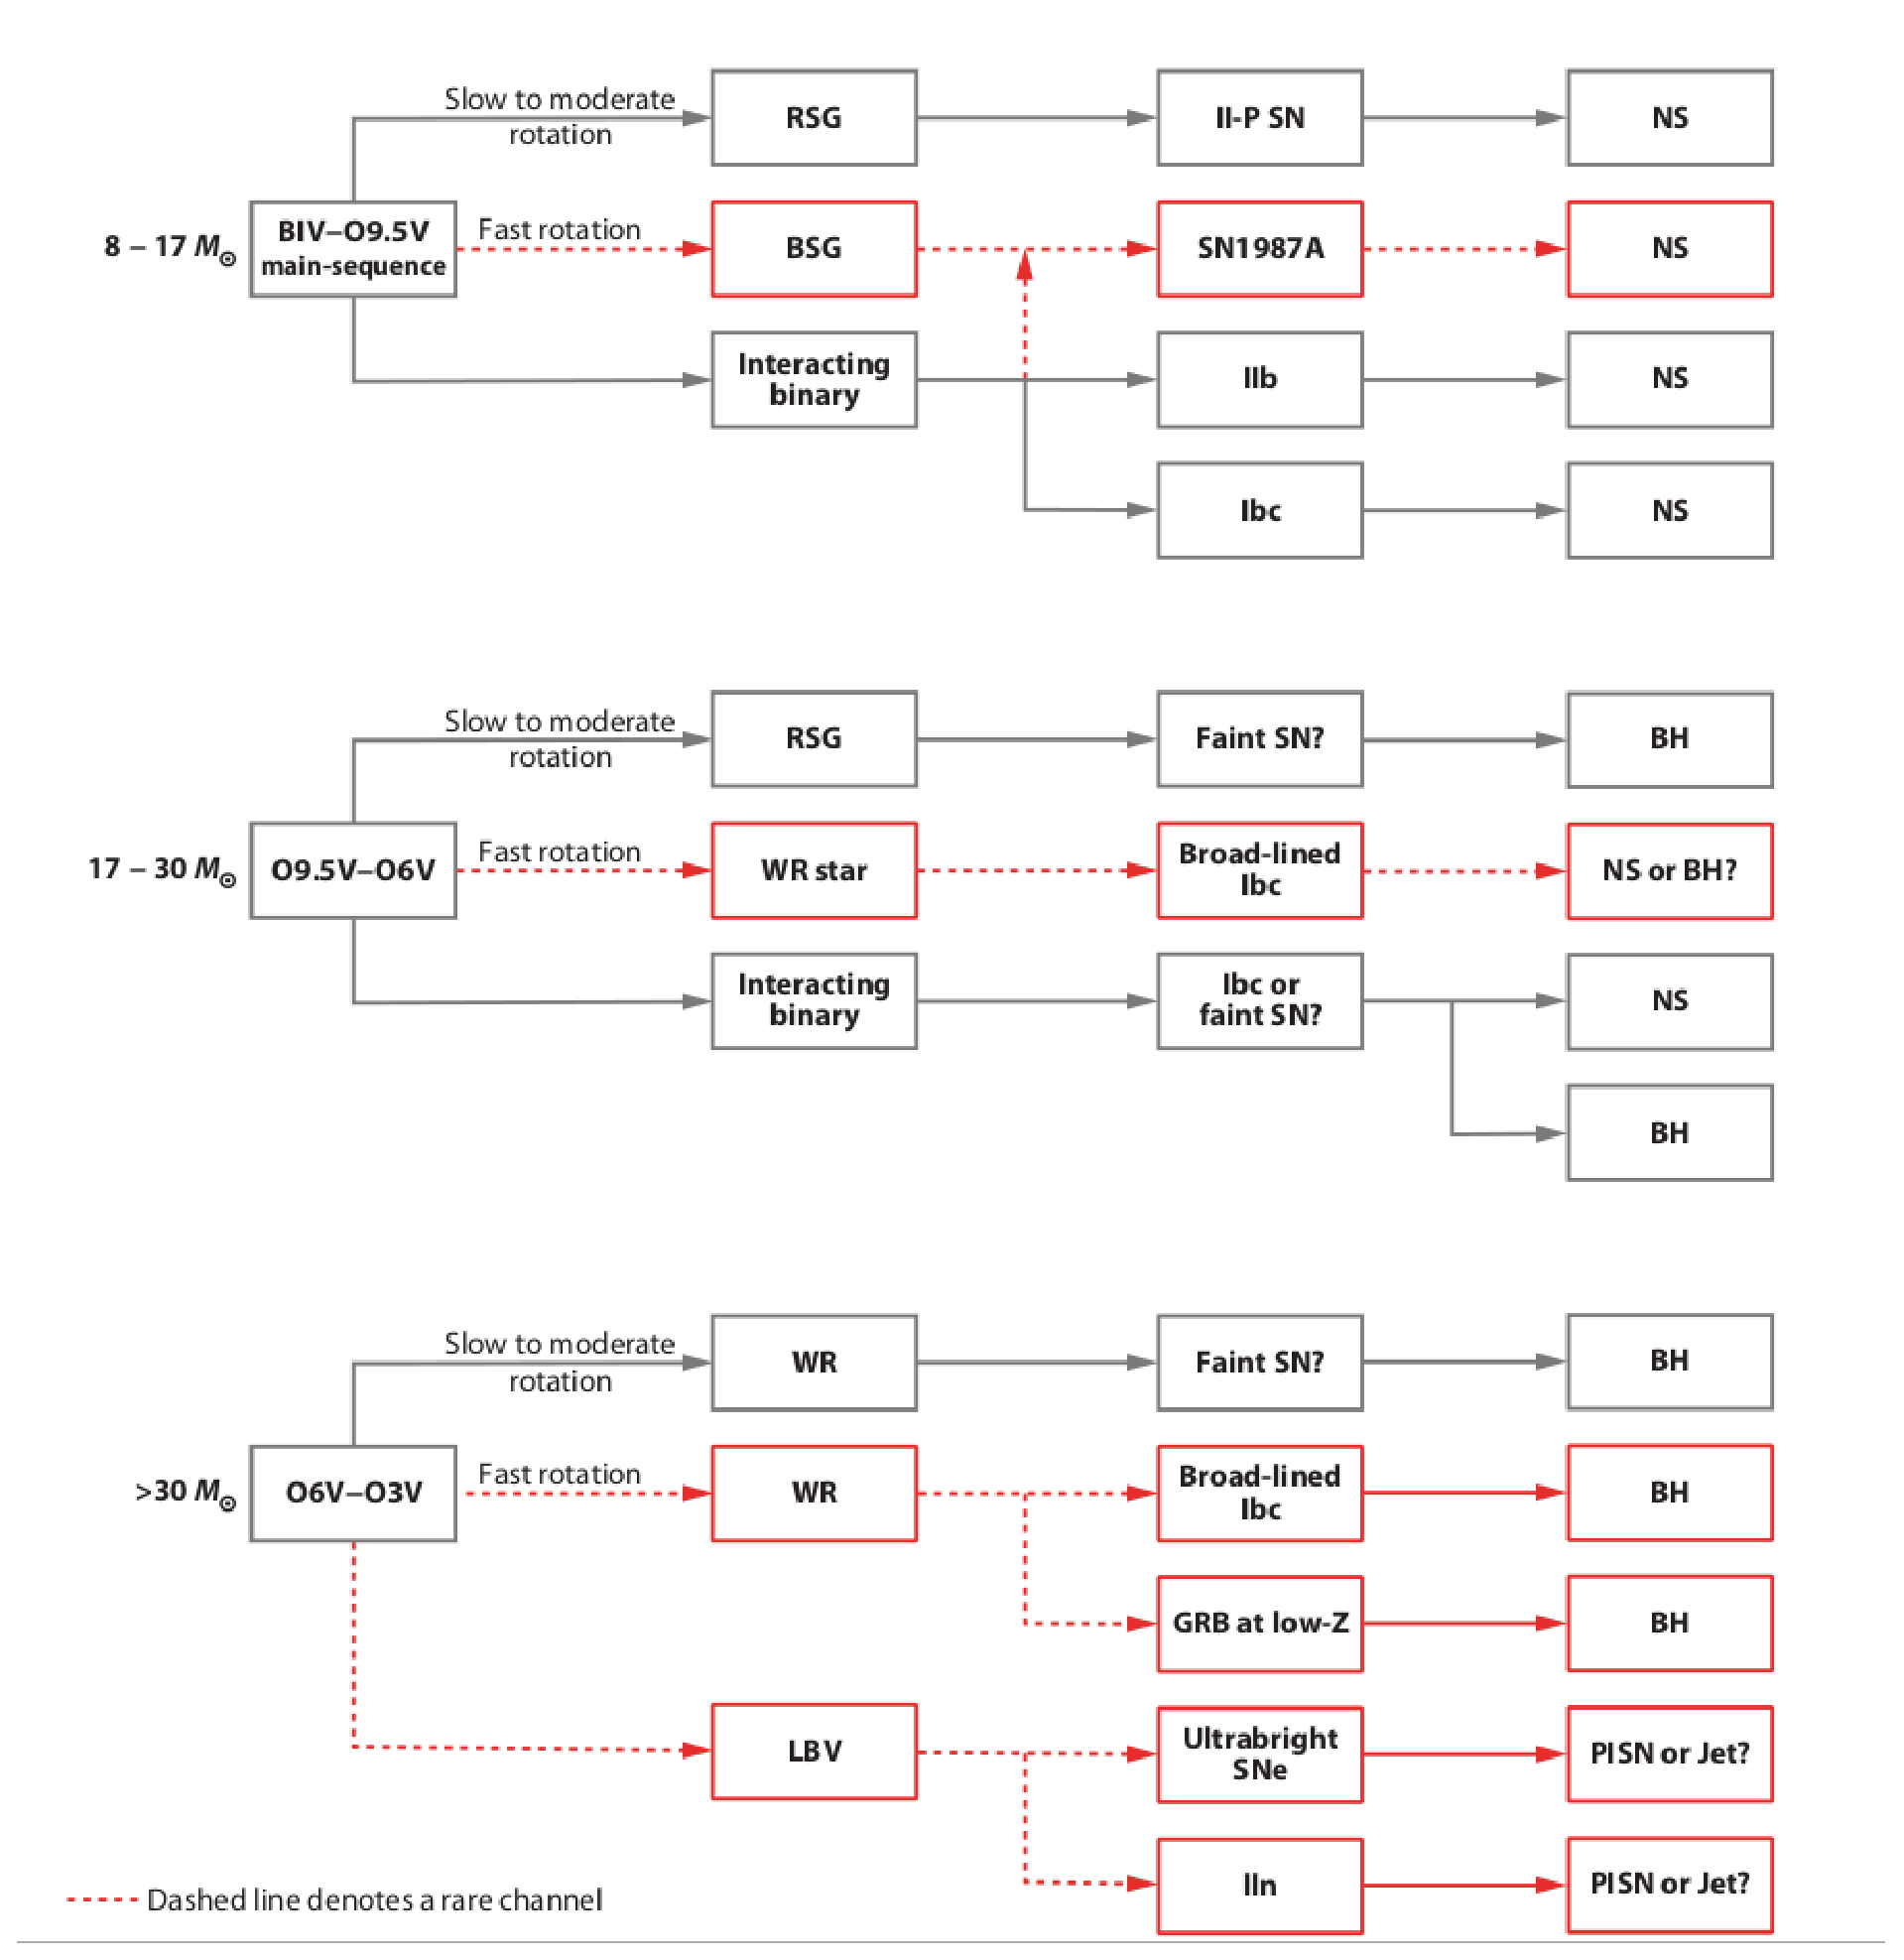
\includegraphics[width=0.65\textwidth]{intro/Smartt09fig12}
 \caption[Endpoints of massive stars]{The evolutionary diversity of the end points of massive stars and their associated observed SN classification. Figure reproduced from~\cite{Smartt09}. Acronym definitions: RSG, red supergiant; BSG, blue supergiant; LBV, luminous blue variable; WR, Wolf-Rayet; NS, neutron star; BH, black hole; GRB, gamma-ray burst; PISN, pair-instability supernova.
 Note that in~\citep{Smartt09}, and hence in this illustration, the upper mass limit of a star which becomes a RSG is 30\,M$_{\odot}$ rather than the 40\,M$_{\odot}$ adopted here.
 \label{fig:SNe-Smartt}}
\end{figure}

% subsection death (end)
% section the_life_of_a_red_supergiant (end)

\section{Observations of RSGs at Home and Abroad} % (fold)
\label{sec:rsg_observations}

Red supergiant (RSG) stars are massive, bright, evolved stars located in recent star-forming environments.
As mentioned above, any star with an initial mass 8~$<$~M/M$_{\odot}<$~40 is expected to spend a portion of its life cycle as a RSG~\citep{2000A&A...361..101M,Massey03, 2007ARA&A..45..177C, Meynet11}.
As RSGs are so luminous, these objects can be studied in external star forming galaxies supplemented of course by more detailed studies of individual stars within our own Galaxy.
However, before one can study RSGs they need to be accurately identified and classified. In Section~\ref{sub:selection_of_rsgs} I deal with how this can be achieved and then highlight some of the key observational results from Galactic and extragalactic studies of RSGs in Section~\ref{sub:galactic_and_extragalactic}.

\subsection{Identification and Classification of RSGs} % (fold)
\label{sub:selection_of_rsgs}

The classification of stars is based on the morphology of their optical spectra, with particular focus upon the absorption lines of hydrogen and other elemental features such as helium and calcium.
RSG stars have spectral type K or M, classified as such based on the appearance of strong molecular lines arising from their cool atmospheres.
Additionally, cool main sequence dwarfs and evolved giant stars also have spectral type K or M.
To distinguish between these populations of stars, luminosity is taken into account.
The luminosity of a star ($L$) is given by the equation,

\begin{equation}
    L = 4\pi R^2\sigma_{SB}T_{\rm eff}^4
\end{equation}

\noindent where $R$ is the radius of the star, $T_{\rm eff}$ is the effective temperature of the star and $\sigma_{SB}$ is the Stefan-Boltzmann constant (which in Chapter~\ref{ch:janal} is defined as one of the fundamental equations of a star).

For a given spectral type the effective temperature of a star is roughly constant, therefore, luminosity is dependent solely upon the radius of the star.
The largest and most luminous stars, the supergiants, are labelled as class~\1, giants as class~\3 and dwarf or main sequence stars, with the smallest radii and hence the lowest luminosity, as class~\5.

In general, spectral features which are sensitive to luminosity are directly related to the physical size of the star rather than a product of the luminosity.
Supergiants have large extended atmospheres; hence, their radii are considerably larger than the more compact dwarfs and giants.
This distinction in physical size of stars results in various characteristic spectral features which are used to determine luminosity class.
In the optical regime, there are various different luminosity class indicators.
For K-type stars, the ratio of the Y\,\2 (4376\,\AA) line with Fe\,\1 (4383\,\AA) or the morphology of the Ca\,\2 H and K lines (for early K-type stars) are some of the most prominent~\citep{b:GrayCorbally}.
While for M-type stars, a system of molecular TiO lines centred on 5000\,\AA ~or the negative luminosity effect of the Ca\,\1 (4226\,\AA) line are clear indicators of luminosity~\citep{b:GrayCorbally}.
In the infrared, the 0-0 band of the CN molecule is the main luminosity discriminator at $\sim$1.1\,$\mu$m for both K- and M-type stars~\citep{b:GrayCorbally}.


% I want to include a section about why these lines change with luminosity class but I'm struggling to find reasons ...
%These features are sensitive to luminosity for a many different reasons. For example, the CaII H \& K lines in supergiants display broad wings, whereas in dwarfs and giants, the lines are narrower.
%Diminishing Stark effect is more extended atmospheres~\citep{b:GrayCorbally}

%Eg. lower densities and pressures cause atomic species with low ionisation energies to be pushed more towards an ionised electron + ion

Distinguishing between dwarfs, giants and supergiants for a given spectral type is important as these stars are different in terms of their stage of evolution and mass.
RSG stars are young, evolved stars which are fusing helium or heavier elements in their cores.
In contrast, dwarf M- and K-type stars are low mass, old stars which are still in the core hydrogen fusion stage.
Giant M- and K-type stars are evolved stars of intermediate mass and intermediate age currently on the asymptotic giant branch (AGB).
The exact divide between AGB stars and RSGs stars is, like all classification sequences which attempt to bin a continuous range of data, somewhat ambiguous and great care must be taken to separate these classes of stars.

The most effective method of classifying stars is to obtain spectroscopic observations which cover some of the important diagnostic luminosity indicators with sufficient resolution to distinguish between unique observational signatures.
In the optical regime, RSGs spectra are dominated by absorption by TiO, which can be seen in all the M- and K-type spectra (illustrated in Figure~\ref{fig:RSGoptical}.
However, spectroscopic observations are expensive.
In the absence of spectroscopic observations, the selection of stars, in general, made based on broad band photometry.
% This section will describe some of the various methods used to isolate a population of stars using magnitudes derived from broad band filters.
Isolating a population of stars using photometric selection techniques is important as photometry can target a large number of stars with a relatively small amount of observing time which can be used to optimise follow up observing programmes to target specific types of stars.

 \begin{figure}
 \centering
 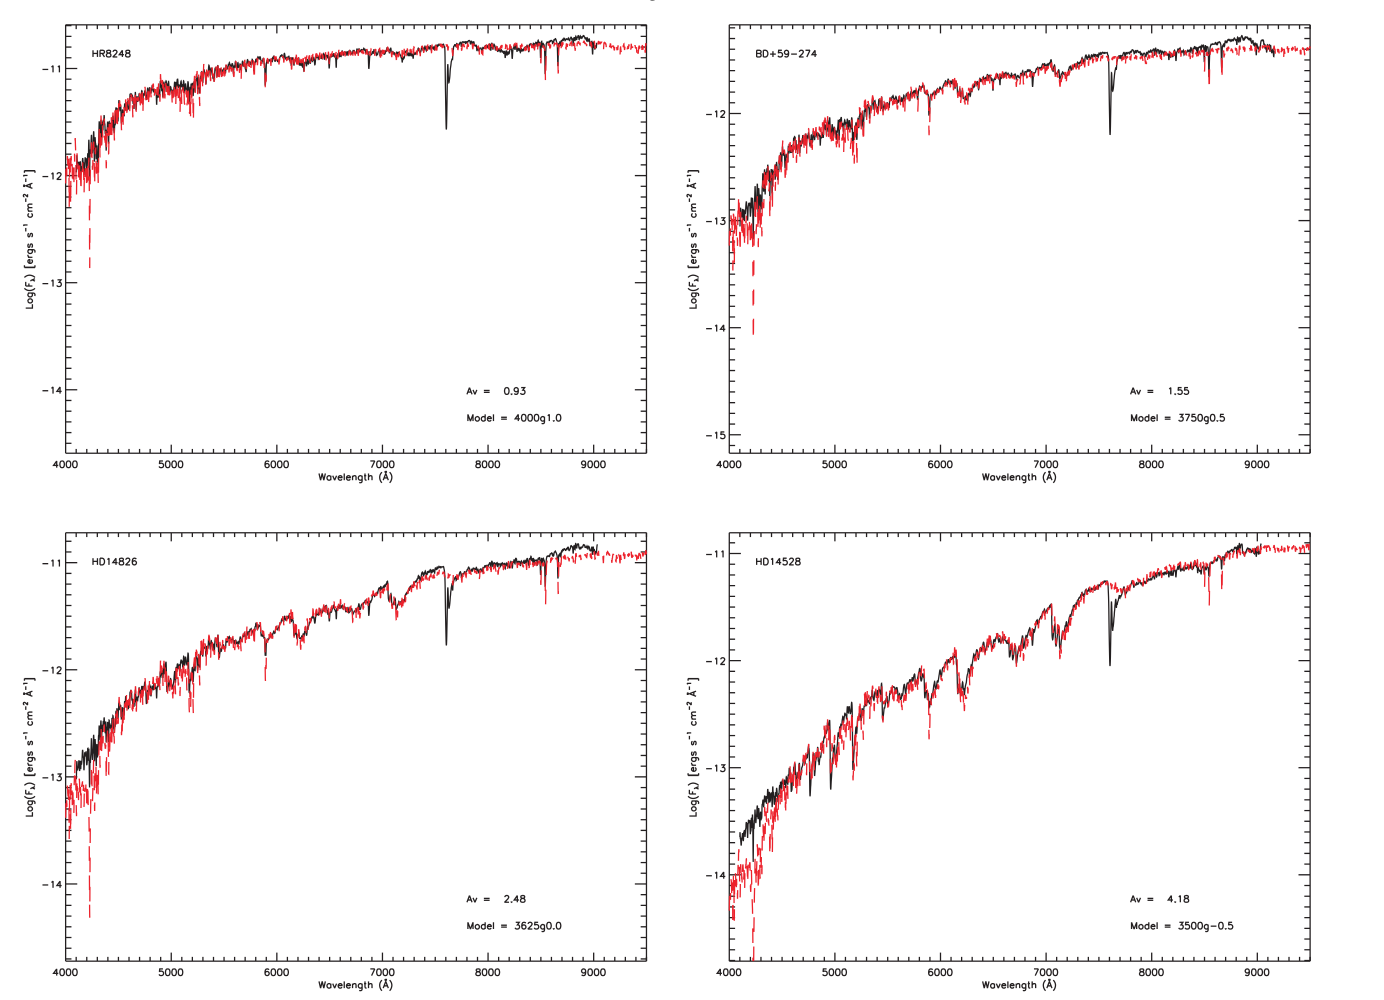
\includegraphics[width=\textwidth]{intro/Levesque_Fig1}
 \caption[Optical spectra of four RSGs from~\citeauthor{Levesque05}]{Optical spectra of four Galactic RSGs from~\cite{Levesque05}, with wavelength in \AA ngstrom on the abscissa shown against the logarithm of observed flux on the ordinate, illustrating that these spectra are dominated by the broad absorption from the TiO molecule.
 Observed spectra are shown in black with an associated best-fit model spectrum in red.
 A$_{\rm V}$ value shown in each figure refers to the amount of ``reddening'' applied to each model spectrum to fit the observations and the number below this indicates the best-fit model effective temperature in Kelvin and the logarithm of the surface gravity in c.g.s units. (For a discussion on how this apparent change in temperature in the optical is related to the appearance of the TiO features in optical spectra of RSGs see Chapter~\ref{ch:ngc6822}.)
 The four panels shown here demonstrate the varying appearance of the TiO features present in RSGs, from top to bottom, left to right:
 HR\,8248 (K1\,I),
 BD\,+59\textdegree274 (M1\,I),
 HD\,14826 (M2\,I) and
 HD\,14528 (M4.5\,I).
 \label{fig:RSGoptical}}
\end{figure}

Colour-magnitude diagrams (CMDs), which are essentially an observational form of the H--R diagram, are often used to isolate particular types of stars.
Colour is defined as the difference between two magnitudes at different wavelengths.
Essentially, a colour traces the shape of the spectrum of the star (which is defined to first order by the effective temperature), and the brightness of a star in a given filter (magnitude) can be used to approximate luminosity.
Therefore, theoretically a CMD should allow for the separation of a population of stars with distinct luminosities and temperatures in the same way as a H--R diagram.
The situation is simplified in the case of the RSGs as these stars are expected to be among the brightest in a stellar population.
However, this method assumes that the sample consists purely of one population of stars at a fixed distance.
When a population of stars is distributed over a significant range of distances, a brighter star with a larger distance is degenerate with a nearby fainter star.
In addition, dust extinction can affect the colours of stars which can cause a star with a bluer colour which is significantly extincted by dust to appear as a redder star with a smaller contribution from extinction.

An example of an optical CMD of NGC\,6822 is given in Figure~\ref{fig:CMD}.
In this figure one can see large scale structures arising as different types of stars distinguish themselves based on their properties.
However, this figure also demonstrates some of the potential issues with using these types of diagrams to select targets.
The large feature at $B-V \sim$~1.0 is attributed to foreground contaminants.
RSGs are found on this figure at the tip of the reddest plume with $B-V >$~1.5.

\begin{figure}
 \centering
 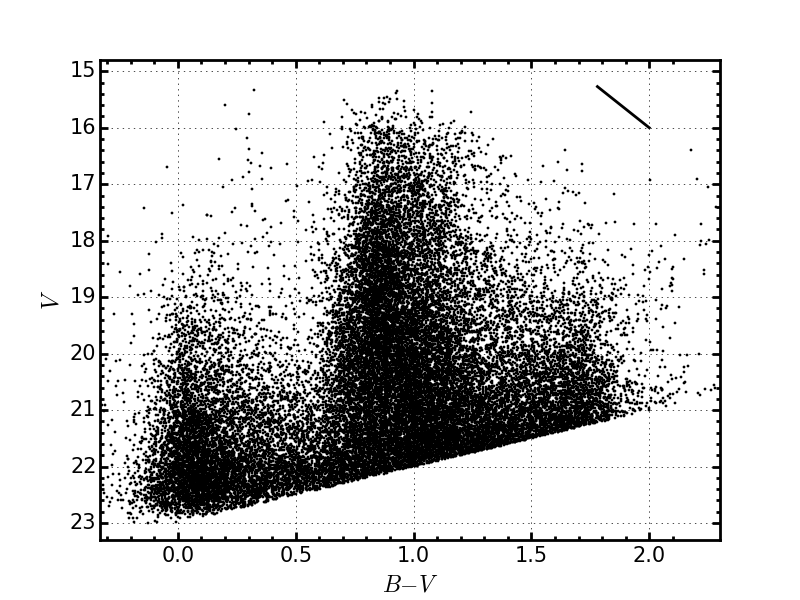
\includegraphics[width=0.65\textwidth]{intro/NGC6822_bv_CMD}
 \caption[Optical colour-magnitude diagram of NGC\,6822]{Optical colour-magnitude diagram (CMD) of NGC\,6822, in which the apparent V-band magnitude $V$, is plotted against $B-V$ colour.
This figure illustrates how CMDs can be used to separate stars based on spectral type. Redder colours generally indicate later spectral types (however, these colours can be strongly affected by interstellar and circumstellar extinction).
This figure also demonstrates that CMDs have inherent degeneracies between different populations of stars.
 \label{fig:CMD}}
\end{figure}

To break the degeneracy between luminosity and distance as well as distance and reddening, one can use colour-colour diagrams (CCDs).
Using multiple colour diagnostics can isolate stars to a greater degree when compared with CMDs.
\cite{1998ApJ...501..153M} show that at a given $V-R$ colour, the $B-V$ colour of a star is sensitive to the surface gravity.
Therefore, RSGs can be isolated from other stars of similar $B-V$ colours owing to their low surface gravity.
An example of such a CCD  is shown, again for NGC\,6822, in Figure~\ref{fig:CCD} where one can clearly see the distinction between low surface gravity RSG stars (with slightly redder $B-V$ colours) and the dwarf high surface gravity stars.

\begin{figure}
 \centering
 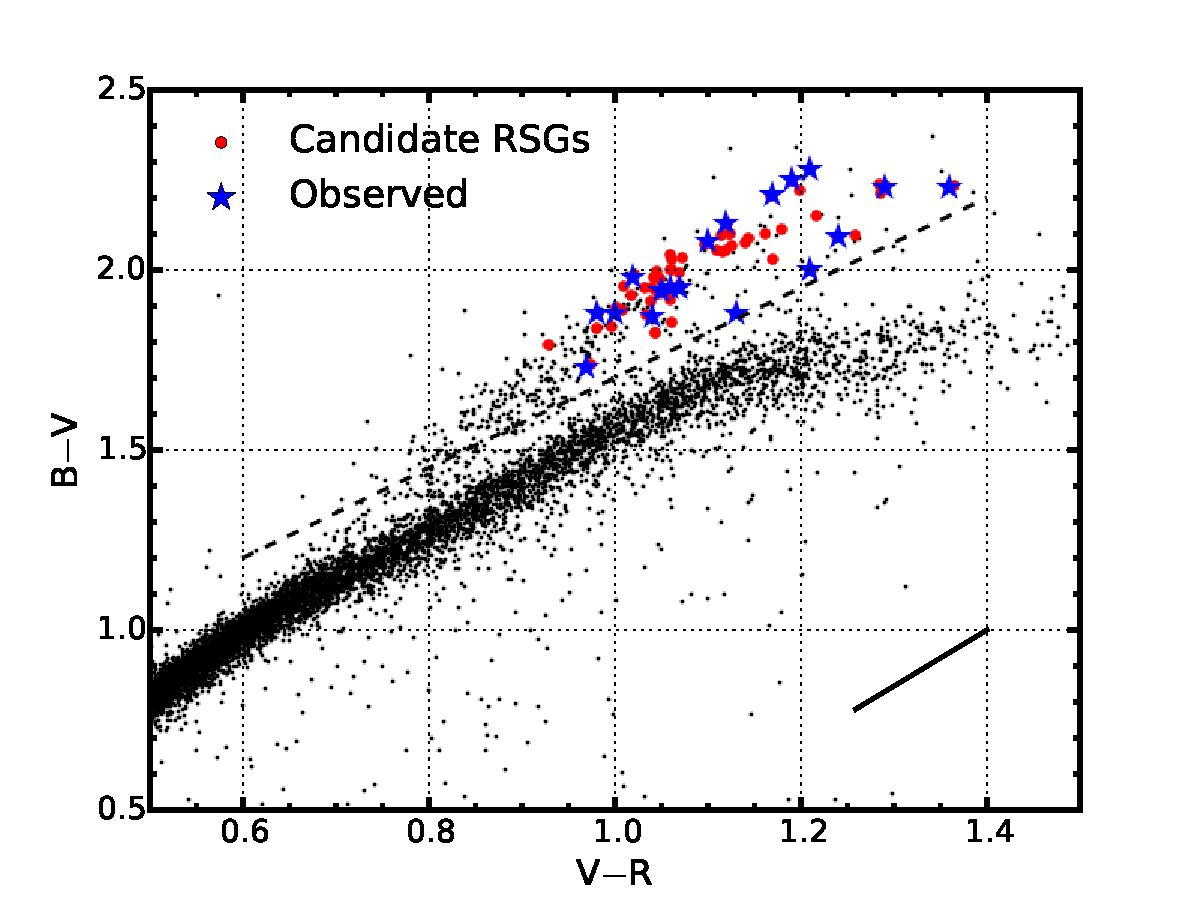
\includegraphics[width=0.65\textwidth]{intro/N6822_bvr}
 \caption[Optical $B-V$, $V-R$ colour-colour diagram]{Optical colour-colour diagram (CCD) of NGC 6822. This figure illustrates the surface gravity dependence of the $B-V$ colour at a given $V-R$ colour where the dashed line separates the population of RSGs from stars with similar spectral types.
 \label{fig:CCD}}
\end{figure}

The selection of RSGs is typically done using a $B-V$, $V-R$ CCD as this diagram has had much success in selecting RSGs and is known to contain a small number of contaminants~\citep[e.g.][]{1998ApJ...501..153M,MasseyOlsen03,Levesque05,Levesque06,2012AJ....144....2L,2015ApJ...803...14P}.\textbf{more examples ...}
However, a potential issue with these diagrams as we move to extragalactic systems is that RSGs are known to reside in dense regions and/or clusters with many bluer, younger stars.
When viewing these stars in the optical, the colours from RSGs could potentially be contaminated to bluer colours by the blue stars which also reside nearby.
In a $B-V$, $V-R$ diagram, this contamination would affect the completeness of the population of RSGs selected.
To quantify this would require a comparison between the $B-V$, $V-R$ selection method with another known selection method and an analysis of the locations of the potentially contaminated RSG stars.
A potential solution to this problem would be to select RSGs based on their near-IR colours, which is where these stars are brightest and hence would be less subject to contamination to nearby blue objects.
% This argument could be reversed and in the near-IR we could push blue stars towards our RSG targets. Would this be a problem?

Working in the near-IR, authors have used the J, J-K CMD~\citep[e.g.][]{2000ApJ...542..804N,2006A&A...452..195C,Neugent12,2015ApJ...803...14P} to select RSGs and asymptotic giant branch (AGB) stars and much work has been done in identifying contaminants and the parameter space where individual populations reside in~\citep{2006A&A...452..195C}.
As mentioned above, the main contaminants with this selection method are foreground dwarfs.

In the mid-IR, authors have used the [3.6] - [4.5] CMD to distinguish between RSGs and various types of AGB stars~\citep{2006AJ....132.2034B,2014A&A...562A..75B,2015A&A...584A..33B,2015ApJ...800...51B,2015A&A...578A.100W} and using these longer wavelengths has proved a useful tool to study the dust properties of these cool stars~\citep{Beasor-prep}.

% subsection selection_of_rsgs (end)


\subsection{Galactic and Extragalactic studies} % (fold)
\label{sub:galactic_and_extragalactic}

The intrinsic brightness of RSGs, particularly in the near-IR, makes these stars popular candidates for observations within and without the Galaxy.
Studies of Galactic RSGs are used to test theories of stellar evolution and estimate fundamental stellar parameters such as radii, masses and distances.
Galactic RSGs are also a natural starting point for extragalactic studies of larger populations of RSGs.
Extragalactic observations have identified populations of RSG stars in a large range of galaxies within the Local Group and (in rarer cases) out to larger distances~\citep[e.g.][and see Chapter~\ref{ch:ngc55}]{Elias85,Humphreys86, Massey06, 2007AJ....134.2474M, Groenewegen09,Massey13,2015ApJ...805..182G}.
These studies provide important results on RSGs in different environments.

% \subsubsection{Fundamental Parameters in Galactic RSGs}\label{Galactic RSGs}

RSGs are intrinsically rare within stellar populations given their masses, and consequently, short lifetimes.
Within the Galaxy there are examples of prominent individual RSGs such as $\alpha$ Orionis (Betelgeuse), VY Canis Majoris and Antares which have gained considerable attention for countless years.\footnotemark
In addition to individual RSGs there are examples of Galactic (and extragalactic) young massive clusters (YMCs) whose light output is dominated by RSGs and contain tens of these objects~\citep{2014ApJ...788...58G}.
Examples include, the {\it h} and $\chi$ double cluster and more recently discovered clusters such as  red supergiant clusters 1, 2 and 3 and Alicante 8~\citep[RSGC01, RSGC02, RSGC03;][respectively; \citealt{2010A&A...513A..74N}]{2006ApJ...643.1166F,2007ApJ...671..781D,2009A&A...498..109C}, each containing a large concentration of RSGs.

\footnotetext{\cite{2003UppOR..59...51R} suggested that cave markings in Germany dating to around 30\,000\,BCE represented the constellation Orion, of which Betelgeuse is part of.}

Research into individual Galactic RSGs typically is concentrated on estimating structural or dynamical properties of atmospheres or on circumstellar material surrounding these stars where one can test detailed stellar evolutionary and atmospheric models against high quality observations~\citep[e.g.][]{2014A&A...561A..15C}.
A useful reference to obtain an overview of what research is being conducted on individual RSGs in the galaxy is~\cite{2013EAS....60.....K}, the conference proceedings for an entire workshop centred around Betelgeuse.

Observations of Galactic RSGs reveal that they have large mass-loss rates
\citep[10$^{-(6\pm 1)}$\,M$_{\odot}$\,yr$^{-1}$;][]{Danchi94, Richards13,2016AJ....151...51S} and extended circumstellar environments~\citep{Smith01,2014MNRAS.437L...1W} which may contain masers~\citep[e.g.][]{Schuster06,2012ApJ...744...23Z}.
Mass loss during this phase of evolution is critical for the understanding of subsequent evolutionary stages as well as understanding SN progenitors.
For example, the remnant of SN 1987A displays loops which are thought to have originated in mass loss events during the RSG phase of evolution of its progenitor star~\citep[][and references therein]{Humphreys13}.
Galactic RSGs act as an important sample to study and understand the mechanisms and rates of mass loss, as extragalactic observations are unable to resolve the structures which can be seen in nearby Galactic stars.

One of the main uncertainties with studies of these nearby stars are the relatively poorly constrained distances e.g. Betelgeuse~\citep[197\,$\pm$\,45\,pc;][]{Harper08} and VY CMa
\citep[$\sim$1300\,$\pm$\,120\,pc;][]{Wittowski12,2012ApJ...744...23Z} which are partly attributed to variations of surface structure affecting the stellar photocentre~\citep{2011A&A...528A.120C}.
However, this affect is likely to be on the 0.1\,AU scale and cannot account sufficiently for the large error in the distance determination, the origin of which remains elusive.
In order to (partially) remove the distance uncertainty problem, RSGs can be observed in Galactic clusters of known distances~\citep[e.g.][]{Humphreys78, Mel'Nik95,2014ApJ...788...58G}.
%% MS fitting, observe spectral type and fit cluster onto a HR diagram to estimate the absolute magnitude, distance modulus
This technique is useful to study large populations of RSGs which can be used to test theories of star formation and models of RSGs and their atmospheres.

% \subsubsection{Extragalactic Studies and Results}\label{extragalactic RSGs}

Extragalactic studies of RSGs have the advantage that it is possible to accumulate large samples of RSGs, at a fixed distance, with which to test stellar evolution theories and estimate stellar parameters.
By using the different environments available in the Local Group, studies of extragalactic RSGs can probe a wide range of host galaxy parameter space.
For example, M31 (Z$>$1.0Z$_{\odot}$ in the central regions), a massive, metal-rich spiral galaxy and the Wolf-Lundmark-Melotte (WLM; Z=0.1Z$_{\odot}$), a dwarf irregular, metal-poor galaxy, both contain a significant population of RSGs.

Through an analysis of RSGs in different metallicity environments, some authors have reported that the average spectral type of a RSG population is dependent upon metallicity~\citep{Elias85, MasseyOlsen03, 2012AJ....144....2L}, where lower metal abundances give rise to earlier average spectral types.
In addition to this, RSGs can be used to measure abundances in Local Group galaxies, which yield important results by mapping metallicity gradients.
This work had typically been done using high-resolution spectra at near-IR wavelengths~\citep{Cunha07, Davies09a,Davies09b}.
However, in order to optimise these studies,~\cite{2010MNRAS.407.1203D} adapted a method for determining the chemical properties of BSG stars in the optical
\citep{2008ApJ...681..269K,2010AN....331..459K}, to RSGs in the near-IR.

These studies exploit that fact that even though RSGs are evolved objects, for massive stars, the hydrogen-burning lifetime is short~\citep[just over 25\,Myr for a 8\,M$_{\odot}$ star and consequently shorter for higher mass stars][]{2012A&A...537A.146E}.
Therefore, although RSG stars are in an evolved state, they are in actual fact still remarkably young stellar objects ($<$30\,Myr old, as subsequent generations of nuclear fusion are significantly shorter than the time scale for hydrogen fusion).
Given the fact that these stars are very young, in general they have not had the time to travel a significant distance from their birth place.
Therefore, their chemical composition must closely match that of their surrounding environment (accounting sufficiently for a certain amount of nuclear processing).
This means that studies of RSGs in extragalactic environments can probe the present day metallicities of their surrounding environments which are comparable to H\,\2 region studies (see Section~\ref{sec:chemical evolution}).

In addition to their young ages, RSGs are also intrinsically attractive objects to study at near-IR wavelengths.
% There are many reasons to study RSG stars at near-IR wavelengths.
From a technological point of view, the next generation of optical-infrared telescope (e.g. European Extremely Large Telescope, Thirty Metre Telescope, James Webb Space Telescope) will be optimised for studies in the near-IR; therefore, in order to make the best use of these facilities in the future, we must refine and optimise our observational strategy on facilities today.

There are also many intrinsic properties of RSGs which make  which make them desirable objects to study in the near-IR.
As noted earlier, RSGs are among the most luminous objects in any star-forming galaxies and, given their cool atmospheres, the peak luminosity for RSGs is $\sim$1.1\,$\mu$m.
Coupled with this is the fact that near-IR observations are less affected by dust obscuration which is important as, by definition, RSGs are dusty objects owing to their high mass-loss rates.
Therefore, near-IR observations are the optimal wavelength to observe RSG stars at large distances.

Measurements of the temperatures of RSGs have also provided insight through using observations of extragalactic RSGs in the near-IR.
The temperatures of RSG stars have been subject to debate for many years which again is likely a product of their complex atmosphere and surface structure.
There are many methods by which to estimate the effective temperature of a RSG star.
The most popular of which is to fit the spectral energy distribution (SED) of the star with 1D model atmospheres~\citep{Levesque05,Levesque06}.
However,~\cite{2013ApJ...767....3D} demonstrated that observations fitting models around the BVRI region, where molecular TiO lines dominate the absorption, result in a systematically lower temperature compared with fitting the line-free continuum regions of the SED.
This is as a result of the TiO molecular line forming higher in the atmosphere of the star than the continuum.
This means that fitting the TiO region and assuming that the best fitting effective temperature is representative of the entire SED is not a good assumption.
\cite{2013ApJ...767....3D} advocate using the entire SED \textit{except} those regions dominated by the TiO absorption features.
Estimating temperatures of extragalactic RSGs will be an important test for stellar evolution models and an excellent way in which to test models at different metallicities and in different environments.
\cite{2015ApJ...803...14P} highlighted the interesting result that the temperature of RSGs in different environments appears to be insensitive to the metallicity of the RSG. (This result is presented and commented upon in Chapter~\ref{ch:ngc6822})

In summary, I have highlighted some of the ways in which one can take measurements of RSGs in both at home (in our own Galaxy) and abroad (in external galaxies).
Owing to various factors I have demonstrated that studies in the near-IR can have a significant impact on the understanding of RSGs and their environments.
RSGs and massive stars in general play a key role in distributing material throughout their host galaxies and understanding the physical process which affect these environments is key to furthering studies of galactic chemical evolution.



% section observations_of_red_supergiant_stars_at_home_and_abroad (end)

\section{Chemical Evolution of Galaxies as Probed by Red Supergiant Stars} % (fold)
\label{sec:chemical evolution}


The evolution of galaxies is a vast area of study which can be broadly split up into three main fields: dynamical, thermal and chemical evolution.
%In reality these topics depend upon each other, but given certain crude approximation can to an extent be studied independently.
The chemical evolution of galaxies governs the origin and distribution of elements within the host galaxy.
This evolution principally depends upon galaxy and star formation where
the initial distribution of the chemical elements is defined by how the galaxy is formed.
Star formation acts to alter these quantities by creating, redistributing and removing chemical elements from the interstellar medium (ISM).

The lowest mass stars remove elements from the ISM by storing their gas and never evolving off the MS.
Stars massive enough to evolve off the MS eject some mass during an AGB phase, but subsequently end their lives by removing elements from the ISM as passively cooling white dwarf stars.
%These stars could also end up as Type Ia SNe
More massive stars undergo large amounts of mass loss during all phases of their evolution and end their lives by exploding as CCSNe, both of which act to alter the chemical composition of their surrounding gas clouds.

All three of these processes are important to take into account when studying how galaxies chemically evolve over time.
However, quantifying contributions from these processes, complicated by a minefield of caveats and uncertainties.

Extragalactic observations of fundamental properties of galaxies play important roles in refining theories of galaxy formation and evolution.
The mass-metallicity relationship~\citep[MZR;][]{Lequeux79} of galaxies relates two fundamental parameters of galaxies.
The stellar mass represents the amount of gas which star formation has removed from the ISM, whereas the present day galaxy metallicity represents how star formation has altered the initial ISM.
Various authors have shown that galaxy mass is proportional to metallicity
~\citep{Tremonti04, Maiolino08,Kewley08}, Figure~\ref{fig:MZR} shows such a result.
This relationship can be interpreted by considering multiple factors.
In low-mass galaxies, outflows and SNe have a greater affect on the amount of material ejected from the host galaxy into the intracluster medium, owing to their shallower potential wells~\citep[e.g.][]{Tremonti04}.
Additionally, low-mass galaxies represent an early stage in Galactic evolution and hence, these galaxies have not had time to process their gas into stars.
As the host galaxy evolves, subsequent episodes of star formation increase the metal content of the galaxy~\citep[e.g.][and references therein]{Maiolino08}.


\begin{figure}
 \centering
 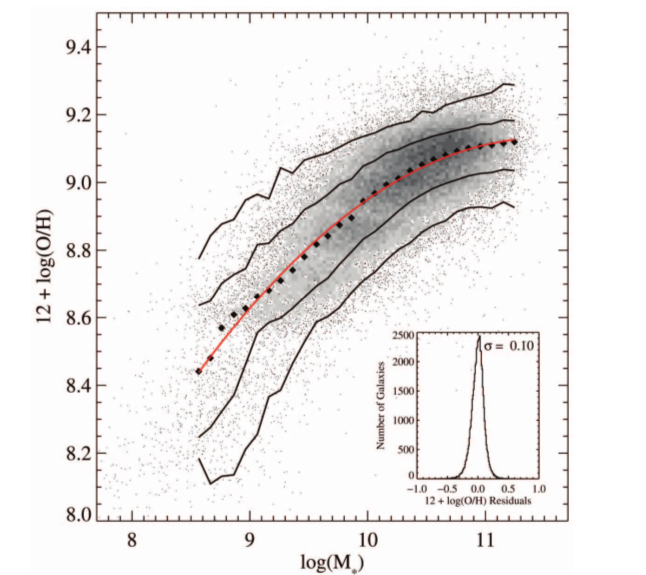
\includegraphics[width=0.65\textwidth]{intro/MZR}
 \caption[\citeauthor{Tremonti04} Mass-metallicity relationship]{The MZR presented in~\citep{Tremonti04} where the gas metallicities of 53\,000 galaxies from the Sloan Digital Sky Survey (SDSS) were measured using nebular emission lines and where the gas mass is measured using H\,$\alpha$ luminosity.
 This figure shows that there exists a fundamental relationship between galaxy mass and metallicity.
 \label{fig:MZR}}
\end{figure}

MZR observations have typically relied upon ratios of strong oxygen emission lines (usually [O\,\2], [O\,\3] relative to H$\beta$) from H\,\2 regions to estimate metallicities of individual galaxies.
This technique is used owing to its applicability over a large distance range:
\cite{2001MNRAS.323..887C} use this technique in nearby galaxies whereas~\cite{Maiolino08} estimate metallicity using this method in galaxies at z$>$3.
However, these measurements are known to be highly dependent upon the calibration method used~\citep{Kewley08,2008ApJ...681..269K,Bresolin09}.
In order to provide an independent calibration of this method, BSG stars have been used to determine metallicity and abundance gradients in external galaxies~\citep{Kudritzki12}.
In addition to using BSGs, this thesis describes and builds on a method which uses RSGs as abundance probes of external galaxies which can be used to calibrate the MZR by building up large numbers of observations of RSGs in external galaxies.

Independent calibration of the MZR is essential to study how galaxies chemically evolve.
The MZR has been shown to exist in the Local Universe as well as at earlier epochs within many different types of galaxies~\citep[e.g.][]{2011ApJ...730..137Z,2013ApJ...765..140A,2014MNRAS.440.2300C,2014ApJ...795..165S,2014MNRAS.437.3647Y,2015ApJ...799..138S} and is thought to be a ubiquitous property of galaxy formation.

% section chemical evolution (end)


\section{Motivation and Outline} % (fold)
\label{sec:motivation_and_outline}

This thesis aims to develop and expand the use of RSGs as abundance probes in external galaxies with the eventual goal of independently calibrating the MZR of galaxy evolution.
By using state-of-the-art model stellar atmospheres and high quality spectroscopic observations of RSGs, in this thesis I will demonstrate the ability of this analysis method to study large populations of RSGs in external galaxies, measuring not only fundamental stellar parameters in a wide range of different environments, but also using RSGs as probes of how metals are distributed within external galaxies.

In addition, this thesis forms the basis on which all studies of RSGs with the $K$-band multi-object spectrograph (KMOS) will be founded upon.
As I continue to learn about this instrument and make the most of the observations which have been obtained, I find that KMOS can not only be used for chemical studies of galaxies, but also to study the kinematics of massive populations within these galaxies.

RSGs have enormous potential to become important indicators of galaxy metallicity and this project has allowed me to become involved in the early phases of this project.
In addition, with the coming generations of facilities and the realisation that near-IR studies have unique insights and qualities, near-IR spectroscopy (in general) will also become an increasingly prominent tool in the toolbox of the astronomer.
Developing these analysis techniques and techniques of observation today is fundamental to make the best use of upcoming observatories.
The aim of this thesis is to contribute significantly to this development.

This thesis is organised as follows.
In Chapter~\ref{ch:kmos} I describe the principles of spectroscopy and go on to describe KMOS, the instrument which is used extensively in this thesis, and detail the complex data products from this type of instrument.

Chapter~\ref{ch:janal} outlines the underlying physics which is used when constructing stellar model atmospheres and describes the state-of-the-art models which are used to analyse RSG spectra.
This leads on to a description of the analysis technique which is used to measure stellar parameters of RSGs and tests this method on various different data sets.

Chapter~\ref{ch:ngc2100} describes KMOS observations of 14 RSGs within NGC\,2100, a YMC in the LMC, where the chemistry and kinematics of the star cluster are assessed.
Using the analysis routines described in Chapter~\ref{ch:janal} stellar parameters are estimated and compared to previous results. An upper limit to the line-of-sight velocity dispersion is measured for the cluster and the dynamical mass is estimated for the first time.
By combining the individual RSG spectra, I demonstrate that this analysis technique can be used to estimated the integrated properties of unresolved clusters at larger distances at LMC-like metallicity.

Chapter~\ref{ch:ngc6822} describes observations of 18 RSGs in NGC\,6822, a dwarf irregular galaxy in the Local Group with a turbulent past.
I test different strategies for reducing this data and quantify the spatial variations in metallicity within this galaxy, finding a suggestion of an abundance gradient.
I demonstrate that using a simple, closed, chemical evolution model the young and old populations of NGC\,6822 are well explained; an important result as NGC\,6822 displays evidence for recent interactions.
In this chapter I also highlight the result that the temperature of RSGs does not depend upon the metallicity, something which is not predicted by evolutionary models.

Chapter~\ref{ch:ngc55} presents observations of 22 RSGs in NGC\,55, a large spiral galaxy outside the Local Group of galaxies.
Stellar parameters are estimated using the technique described in Chapter~\ref{ch:janal} and I discuss how to optimise the data reduction strategy to obtain results from a challenging data set.
Spatial variations in metallicity are examined and the evolution of NGC\,55 is commented upon.

% Chapter~\ref{ch:mzr} provides a first look at the calibration to the MZR using RSGs in the Local Universe.
% Using the results of the previous three chapters I estimate the MZR from three data points.

Finally, Chapter~\ref{ch:conclusions} presents concluding remarks and provides a first look at the calibration to the MZR using RSGs in the Local Universe.
I build upon this first look calibration by outlining the future work which I will take in this direction.

% \bibliography{../journals,../books}

% section motivation_and_outline (end)